% Chapter 1

\chapter{Groups growth model} % Main chapter title

\section{Introduction}

Social groups, informal or formal, are building mesoscopic elements of every socio-economic system. Their emergence, evolution, and disappearance are at the heart of change in a social system \cite{}. Settlements, villages, towns and cities are formal and highly structured social groups of countries. Their organisation and growth determine the functioning and sustainability of every society \cite{barthelemy2016structure}. Companies are the building blocks of every economy and their dynamics are important indicators of level of development of every economy \cite{hidalgo2009building}. Scientific conferences, as a scientific groups, enable fast dissemination of the latest results, exchange and evaluation of ideas as well as a knowledge extension, and thus are integral part of science \cite{smiljanic2016theoretical}. The membership of individuals in various social groups, online and offline, can be essential when it comes to quality of their life \cite{montazeri2001anxiety, davison2000talks, cho2012tea}. Therefore, it is not surprising that the social group dynamics and their sustainability are at the center of the attention of many researchers \cite{aral2012identifying,gonzalez2013broadcasters, torok2013opinions, yasseri2012dynamics}.\\

The abundance of data enabled the application of methods and paradigms from statistical physics in studying the structure and dynamics of social systems \cite{castellano2009statistical}. The main argument for using statistical physics to study social systems is that they consist of a large number of interacting individuals. Due to this, they exhibit different patterns in their structure and dynamics, commonly known as \textit{collective behavior}. A collective behavior, observed both in physical and social systems, is enforced by a few basic properties of building units and is independent of all other characteristics. The phenomenon is known as \textit{universality} in physics and is commonly observed in social systems such as in voting behavior \cite{chatterjee2013universality}, or scientific citations \cite{radicchi2008universality}. The discovery of universality and scaling in phenomena indicate the existence of universal and straightforward mechanisms that govern the dynamics of a system \cite{}.\\  


The availability of large-scale and long-term data on various online social groups has enabled the detailed empirical study of their dynamics. The focus was mainly on the individual groups and how structural features of social interaction influence whether individuals will join the group \cite{backstrom2006group} and remain its active members \cite{smiljanic2016theoretical, smiljanic2017associative}. The study on LiveJournal \cite{backstrom2006group} groups has shown that decision of an individual to join a social group is greatly influenced by the number of her friends in the group and the structure of their interactions. The conference attendance of scientists is mainly influenced by their connections with other scientists and their sense of belonging \cite{smiljanic2016theoretical}. The sense of belonging of an individual in social groups is achieved through two main mechanisms \cite{smiljanic2017associative}: expanding of the social circle at the beginning of joining the group and strengthening of the existing connections in the later phase. The dynamics of social groups depend on their size \cite{}. Analysis of the evolution of large-scale social networks has shown that edge locality plays a critical role in the evolution of social networks \cite{leskovec2008microscopic}. Small groups are more cohesive with constant membership, while large groups tend to change their active members constantly \cite{PNAS}. Previous research focused on the growth of the single group, the evolution of its social network, and the influence of the structure on its growth. However, how growth mechanisms influence the distribution of members of one social system among groups is still anecdotal.\\

Furthermore, it is not clear whether the growth mechanisms of social groups are universal or system-specific. The size distribution of social groups has not been studied in great detail. Rare empirical evidence of size distribution of groups and communities indicates that it follows power-law behavior \cite{}.  The distribution of the size of the cities and firms has been studied in great detail. Analysis of the sizes of the cities shows that the distribution of all cities follows a log-normal distribution, while the distribution of the largest cities resembles Zipf's distribution \cite{fazio2015pareto}. The scaling behavior was observed in the growth of the companies \cite{stanley1996scaling}, while empirical evidence shows that distribution of company sizes follows log-normal behavior and remains stable over decades \cite{amaral1997scaling}. 

Can we create a unique yet relatively simple microscopic model that will reproduce the distribution of members between groups and explain the differences observed between social systems? French economist Gibrat proposed a simple growth model to reproduce companies' and cities' observed log-normal size distribution. However, the analysis of the growth rate of the companies \cite{amaral1997scaling} has shown that growth mechanisms are different from ones assumed by Gibrat. Analysis of the growth of three online social networks showed that population growth is not determined by the population size and spatial factors, and it deviates from Gibrat's law \cite{zhu2014online}. The growth through diffusion and growth by other means have been used as mechanisms in the model used for prediction of rapid group growth \cite{kairam2012life}. The growth mechanisms of various social groups and the source of the scaling observed in socio-economic systems thus remain hidden.\\

Here we analyze the distribution of formal social groups in two different systems: Meetup online platform and subreddits in the Reddit community. We analyze the scaling behavior of size distributions and distribution of growth rates. Analysis of the dependence of growth rates indicates that growth can not be explained through Gibrat's model. We propose a simple microscopic model that incorporates some of the results of previous research \cite{backstrom2006group}. In our model, the social system grows by adding a constant number of new individuals. The number of groups grows as well, and they overlap in terms of membership, i.e., one individual may be a member of more than one group. An individual can create a new group or join an existing one according to some probability. The choice of the existing group depends on the number of social connections already present. We show that the model can reproduce size distributions and growth rate distribution for both studied systems. We analyze the model and show that it can produce a broad set of distributions depending on the value of model parameters.\\

The paper is organized as follows: in Section \ref{sec:data} we describe the data, while in Section \ref{sec:emp} we present our empirical results. In Section \ref{sec:model} we introduce model parameter and rules. Section \ref{sec:results} we demonstrate that model can reproduce the growth of social groups in both systems and show the results for different values of model parameters. Finally, in Section \ref{sec:con}, we present concluding remarks and discuss our results. 


\section{Data}
We analyse the growth of social groups from two widely used online platforms: Reddit and Meetup. Reddit \footnote{https://www.reddit.com/} enables sharing diverse web content, while Meetup \cite{www.meetup.com} allows people to use online tools to organize offline meetings. Reddit users interact exclusively online through posts and comments. The building elements of the Meetup community are topic-focused groups, such as food lovers or ICT and data science professionals. Due to their specific activity patterns - events where members meet face-to-face - Meetup groups are geographically localised. 

We compiled the Reddit data from https://pushshift.io/. This site collects data daily and, for each month, publishes merged comments and submissions in the form of JSON files. 
Specifically, we focus on subreddits - social groups of Reddit members interested in a specific topic. We select all subreddits active in 2012 and follow their growth from their beginning until 2017. The considered dataset contains 17000 subreddits, with the oldest originating from 2003 and the youngest being from 2017.\\
For each post under a subreddit, we extracted the information about the user-id of the post owner, subreddit-id, and timestamp. We observed the data from $2006$ to the $2017$ year, and for each subreddit and user-id, we selected timestamp when a user made a post for the first time. For our analysis, we chose subreddits still active in $2017$ while removing small subreddits active for less than a month. The resulting dataset contains $304 007$ subreddits and  $36 595 134$ users. \\
For simulation, we extracted data until $2011-12$ and removed all subreddits with a small amount of activity. This reduced the dataset significantly - we obtained only $17 073$ subreddits with $2 195 677$ active users. 

The Meetup data were downloaded in $2018$ using public API. The Meetup platform was launched in 2003, and at the moment we accessed the data, there were more than 240000 active groups. For each group, we extracted information about the date it had been founded, its location, and the total number of members. We focused on the groups founded from $2003$ until $2017$ in big cities such as London and New York, where Meetup platform achieved considerable popularity. We considered groups active at least one month. There were 4673 groups with $831685$ members in London and 4752 groups with $1059632$ members in New York. In addition, we extracted the Id of each member in the group, which allowed us to obtain complementary information about the date a member joined a group. 

From collected data, for each group, we can calculate the number of new members per month and so the group sizes $S_i$ at each time step (month). The growth rate $R_i$ at step $i$ is obtained as logarithm of successive sizes $R = log(S_t/S_{t-1})$. 

%We select two locations, London and New York, and study the formation and growth of groups in these two locations from 2003 until 2017. The total number of groups studied for London is 4000 and 8000 for New York. 
%Potreban je slican opis za Meetup podatke

While these two communities differ in means of communication between their users and activities these users engage in, there are certain common properties that enable us to use same methods to study the growth of these groups and make comparative analysis of their growth. In both communities, users can create new groups and join existing ones. One user can be a member of more than one group/subreddit and there are no limits in the number of groups. For each meetup group we have an information on when an user has joined the group, i.e., we have an information about the group size at every moments. For a subreddit we have a detailed information about users' activity and this we have an information when a user made a first post. This moment is considered as the moment when the user has joined the subreddit and became an active member. In our case we do not consider activity of when a user leaves the group of subreddit, since this kind of information is not available to us. For these reasons, the size of groups we are considering is non-decreasing function. 

\section{Empirical analysis of social group growth \label{sec:emp}}
\begin{figure}[h!]
	\centering
	\includegraphics[width=0.6\linewidth]{Figures/Fig2.png}
	\caption{The number of groups over time, sizes distribution and logrates distribution for Meetup groups created in London from 08-2002 until 07-2017 that were active in 2017 and subreddits created in the period from 01-2006 to the  12-2011 that were active in 2017. }
	\label{fig:data1}
\end{figure}

Figure \ref{fig:data1} summarize properties of the groups in Meetup and Reddit networks. The number of groups grows exponentially over time. Nevertheless, we notice that Reddit has much more groups than Meetup and that Reddit groups are prone to engage more members in a shorter period of time (sizes of meetups range up to  $10^4$, while sizes of subreddits are up to $10^6$). The distributions of group sizes follows the lognormal distribution
\begin{equation}
P(S)=\frac{1}{S\sigma\sqrt{2\pi}}exp(-\frac{(\ln(S)-\mu)^{2}}{2\sigma^{2}})
\label{eq:log} \ ,
\end{equation}
where $S$ is the group size and $\mu$ and $\sigma$ are parameters of the distribution. We used package \cite{powerlaw} to fit Eq. \ref{eq:log} to Reddit and Meetup data and found that distribution of groups sizes for Meetup groups in London and New York follow the same distribution with the value of parameters $\mu= 5.96$, $\sigma = 1.38$. The distribution of sizes of subreddits also has the log-normal shape with parameters $\mu= -1.59$ and $\sigma = 3.99$. Even though these distributions are from the same class, for subreddits we find broader distribution that may resembl power-law distribution. Our strict analysis shown in Supportive Information (SI) confirms that the distribution exhibits a log-normal behavior.  

The lognormal distributions can be generated by multiplicative processes \cite{mitzenmacher2004brief}. If there is a quantity with size $S_i$ at time step $t$, it will grow so after time period $\delta$ the size of the quantity is $S(t+\Delta t) = S(t) r$, where $r$ represents a random process. The Gibrat law states that growth rates $r$ are uncorrelated and do not depend on the current size. In order to describe the growth of social groups, we calculate the logarithmic growth rates defined as $R = log\frac{S_t}{S_{t-\Delta t}}$. According to Gibrat law, the distribution of sizes follow lognormal distribution. For logarithmic growth rates expected distribution is normal, or as it is shown in many studies it is better explained with Laplacian (“tent  shaped“) distribution \cite{mondani2014fat}, \cite{fu2005growth}. In figure \ref{fig:data1} we calculate distributions of logrates for a time period of $\Delta=1 month$. For both networks Meetup and Reddit, logrates are very well approximated with lognormal distribution. The Fig. \ref{fig:data1} shows that logrates depen in the groups size, especially for the smaller and medium size groups. Our analysis of growth of social groups shows that this growth violates the basic assumptions of the Gibrat's law \cite{frasco2014spatially, qian2014origin}, and thus the this growth can not be explained as a simple multiplicative process.\\

We are considering a relatively large time period for online groups. The fast expansion of ICTs led to change of how users how users access online communities. With the use of smartphones the online communities became more available and which led to exponential growth of communities \ref{fig:fig4} and potential change in the mechanisms that influence growth of social groups in these communities. For these reasons we have aggregate groups according to year they were founded for each of the three datasets. For each year and each of the three datasets we calculate the average size of the group $<S>^{y}_{x}$, here $y$ is year and $x$ is the $L$, $NY$ or $R$ depending on the dataset, and normalize the size of the groups. The distribution of normalized sizes is shown in \ref{fig:scale}. All distributions exhibit log-normal behavior. Furthermore, the distributions for the same dataset and different years follow a universal curve with same value of parameters $\mu$ and $\sigma$. The universal behavior is observed for distribution of normalized logrates, shown in Fig. \ref{fig:scale} (bottom panel). This indicates that growth of the social groups did not change due to increased growth of users in online communities, but rather it indicates that the growth is independent on the size of the whole of the system.   

\begin{figure}[!h]
	\centering
	\includegraphics[width=0.8\linewidth]{Figures/Fig1.png}
	\caption{The figure shows the groups' sizes distributions and log rates distributions. Each distribution collects groups founded in the same year and is normalized with its mean value. The group sizes are at the end of 2017. for meetups and 2011. for subreddits. }
	\label{fig:scale}
\end{figure}

\section{Model \label{sec:model}}
Growth of social groups can not be explained with the simple rules of Gibrats law. Previous research on group growth and longevity has shown that social connections with members of a group influence individual's choice to join that group \cite{kairam2012life, zheleva2009co}. However, not only social connections, but also individual's interests and need to discover new content or activity may have an influence on individuals' diffusion between groups. Furthermore, social systems constantly grow since new members join every minute. The growth influences both dynamics of the system \cite{mitrovic2011quantitative, dankulov2015dynamics} and the structure of social interactions \cite{vranic2021growth}. Social groups are constantly created, allowing members to group around common interest or to further solidify their interactions through common activities. Based on these observations, we propose a model of group growth that combines these processes, see in Fig. \ref{fig:fig3}.\\

In our model, we represent a social system as a bipartite network, with two partitions of nodes, users and social group. By definition, the links in bipartite networks exist only between nodes belonging to two different partitions. In our model, the link indicates that the user is a member of a group. Previous studies have used a bipartite growing network model to describe the structure of the social network and its communities \cite{zheleva2009co, leskovec2008microscopic, yang2014structure, ZHANG20136100}. This representation of social system is especially useful in studying overlapping communities, where users can be members of multiple groups. The paper \cite{zheleva2009co} proposed a growing network model where a bipartite (referred to as affiliation) network interacts with the social network, such that users have a preference to the friend’s groups. In our data, we do not have information about explicit friendships. Yet to include diffusion growth of the social networks we assume that a new member links to a small number of individuals already present the in group.

In our model, we allow the growth of both network partitions, figure \ref{fig:my_label}. The partition of users grows through the addition of new users. The groups partition grows through creation of a new group and depends on users' activity. Before joining a group new user makes the link to a randomly chosen node in the social network. This condition allows each user to perform diffusion linking \cite{kairam2012life}. 

At each time step, we add $N_{u}$ new users. Old users are not active in each time step, but we control their activity with parameter $p_{a}$. Active users, new users and a sample of old users that were activate, have an option to create a new group with probability $p_{g}$ or to join one of the existing groups with probability $1-p_{g}$. If a user decides to join an old group, he/she chose with probability $p_{aff}$ to join the social group that is already populated by their friends. That group is chosen according to overlap of friendship connections. This way we mimic social diffusion process. With probability $1-p_{aff}$ a user can join randomly selected group. Through this step we mimic a behavior of users when they prefer to explore their interests or discover a new content or activity. 

Our model is different from one proposed in Ref. \cite{zheleva2009co}. In Ref. \cite{zheleva2009co} when user chooses with probability $p_{aff}$ the group of her friends, that group is chosen randomly from this list. When user decides to chose a group randomly, with probability $1-p_{aff}$, she selects a random group with probability proportional to its size. 
Combination of Preferential attachment leads to power-law shape of the distribution of group sizes \cite{zheleva2009co}.
\\~\\
In the co-evolution model \cite{zheleva2009co}, the evolution of affiliation and social networks are dependent. At each time step new nodes $V_t$ arrive to the network, $V_t$ is from predefined arrival process $N(.)$. At arrival time $t$, the lifetime $a$ of node is sampled from $\lambda e^{-\lambda a}$, so node becomes inactive $t_{end}(v) = t+a$. Parameter is fixed to $\lambda = 0.0092$.  Node decides to go for a sleep during time period $\delta$, so node will wake up at $t+\delta$. The $\delta$ is sampled from $\delta e^ {-\alpha} e^{-\beta degree(v) \delta}$. Parameters are fixed to $\alpha=0.84$, $\beta = 0.002$. \\
At arrival new nodes first make first social linking. Node $v$ chooses friend $w$ with probability proportional to $degree(w)$. Awaken nodes at time $t$, makes social by closing triad two random steps away and they need to  decide the number of groups $n_h$ to join. This is sampled from an exponential distribution $\lambda e^ {-\lambda n_h}$, with mean $\mu^{'} = \frac{1}{\lambda ^{'}} = \rho degree(v) ^ \gamma$, while $\gamma=0.5$.
The user can make new group $h$ with probability $\tau$. Otherwise user joins one of the existing groups. With probability $p_v$, group is chosen through friend, while with probability $1-p_v$ user joins a random group with probability proportional to the group size. The probability $p_v$ is correlated with node degree, $p_v=\eta degree(v)$, where parameter $\eta$ represents the friends' influence on joining a group. \\
The differences between our and co-evolution model are:
\begin{itemize}
	\item the probabilities in our model are fixed, while in \cite{zheleva2009co}, probability that group is chosen from friend is degree dependent, also times when user is active are sampled from exponential distribution, while in our model each user can be active with same probability. 
	\item If user choose group through friend, probability, group is randomly picked up from list of friends' groups, while in our model probability is proportional to number of friends in the group. If user choose random group, it has preference to larger groups, while in our model it is random choice. We also tried random linking as in \cite{zheleva2009co} and it lead to power law degree distribution of groups' sizes. 
	\item In our model first social linking is random, while social linking happens when user joins new group, linking randomly with small sample of group's members 
	\item In our model we allow multiply nodes to be active at each time step, but in single time step each user joins/makes one group. 
\end{itemize}

%With probability, $p_{aff}$ the group is chosen according to the social relations, such that preferred groups are those with more friends (this is different from \cite{zheleva2009co}, they just pick a group from a friend with some probability). 
%Otherwise, the user selects a random group to join 
%(this is different from \cite{zheleva2009co}, they choose a random group with probability proportional to its size; with preferential attachment, group sizes distribution is power-law as presented in their paper).

\begin{figure}[h!]
	%%% OVO JE MOZDA PREVISE PA AKO MISLITE MOZEMO I DA IZBACIMO ili ostavimo samo ovaj donji panel.
	\centering
	\includegraphics[scale=0.5]{Figures/test.png}
	\caption{The top panel shows bipartite (user-group) and social (user-user) network. Filled nodes are active users, while thick lines are new links in this time step. In the social network dashed lines show that users are friends but still do not share same groups. The lower panel shows model schema. \textbf{Example:} user $u_6$ is new user. First it will make random link  with node $u_4$, and then with probability $p_g$ makes new group $g_5$. With probability $p_a$ user $u_3$ is active, while others stay inactive for this time step. User $u_3$ will with probability $1-p_g$ choose to join one of old groups and with probability $p_{aff}$ linking is chosen to be social. As its friend $u_2$ is member of group $g_1$, user $u_3$ will also join group $g_1$. Joining group $g_1$, user $u_3$ will make more social connections, in this case it is user $u_1$.}
	\label{fig:my_label}
\end{figure}

This model can be easily adapted to follow the arbitrary number of new users at each time step. The parameters $p_a$ and $p_g$ determine the number of groups in the network, while with $p_{aff}$ the shape of group sizes distribution can be modified. If  $p_{aff}=0$ the linking mechanism is random and the distribution of groups sizes follow lognormal. With higher affiliation parameter distribution becomes broader, with larger variance. 


\section{Results \label{sec:results}}

For each group, we selected time point when user becomes the member. Looking into whole set of groups during selected time period, we can determine if user is active for the first time (new users) or it is already member of other groups (old user). Also, we can track the number of new groups. To simulate reddit and meetup network, we can approximate some parameters from real data. The time series of the new users can be directly incorporated in the model. Probabilities that old users are active $p_a$ and that new groups are created $p_g$ can be approximated from the data as $p_a = median [\frac{N_{old}(t)}{N(t)}]$, 
$p_g = median [\frac{Ng_{new}(t)}{N_{new}(t)+N_{old}(t)}]$, 
where $N$ is cumulative number of users in the network, $N_{old}$ is number of old active users while $N_{new}$ is number of new active users. The number of new groups is denoted as $Ng_{new}$.
We calculated the following parameters:
Meetup $p_a=0.05$, $p_g=0.003$, for Reddit $p_a=0.1$, $p_g=0.003$. 
We run the simulation with time series of new users, fixed parameters $p_a$ and $p_g$, while we vary affiliation parameter. We discovered that in meetup users are more likely to join groups randomly, the best model fit to data is found for small affiliation parameter 0.1. On the other hand, distribution of sizes for the Reddit network is better approximated with the higher affiliation parameter $p_{aff}=0.9$



\begin{figure}[h!]
	\centering
	\includegraphics[width=0.6\linewidth]{Figures/Fig3.png}
	\caption{}
	\label{fig:fig3}
\end{figure}

\begin{figure}[h!]
	\centering
	\includegraphics[width=0.6\linewidth]{Figures/Fig4.png}
	\caption{}
	\label{fig:fig4}
\end{figure}

\begin{table}[]
	\centering
	\begin{tabular}{c|c|c|c | c|c |c| c| c | c}
		
		paff & 0.1 & 0.2 & 0.3 & 0.4 & 0.5 & 0.6 & 0.7 & 0.8 & 0.9  \\
		\hline
		JS cityLondon & 0.0161 & 	0.0101  &	0.0055 &	0.0027  &	\textbf{0.0016} & 	0.0031 & 	0.0085  &	0.0214 & 	0.0499 \\
		JS cityNY & 0.0097 &	0.0053 & 	0.0026 &	\textbf{0.0013} & 	0.0015 & 	0.0035 & 	0.0081 & 	0.0167 &	0.0331 \\
		JS reddit2012 & - & - & - & - &  0.00074 & 0.00048 & 0.00039 & \textbf{0.00034} & 0.00047 \\
	\end{tabular}
	\caption{Jensen Shannon divergence between group sizes distributions from model (in model we vary affiliation parameter paff) and data. }
	\label{tab:my_label}
\end{table}


\section{Introduction}

Social groups, informal or formal, are mesoscopic building elements of every socio-economic system. Their emergence, evolution, and disappearance are at the heart of change in a social system \cite{}. Settlements, villages, towns and cities are formal and highly structured social groups of countries. Their organisation and growth determine the functioning and sustainability of every society \cite{barthelemy2016structure}. Companies are the building blocks of every economy and their dynamics are important indicators of level of development of every economy \cite{hidalgo2009building}. Scientific conferences, as scientific groups, enable fast dissemination of the latest results, exchange and evaluation of ideas as well as a knowledge extension, and thus are an integral part of science \cite{smiljanic2016theoretical}. The membership of individuals in various social groups, online and offline, can be essential when it comes to the quality of their life \cite{montazeri2001anxiety, davison2000talks, cho2012tea}. Therefore, it is not surprising that the social group emergence and evolution are at the center of the attention of many researchers \cite{aral2012identifying,gonzalez2013broadcasters, torok2013opinions, yasseri2012dynamics}.\\

The abundance of data enabled the application of methods and paradigms from statistical physics in studying the structure and dynamics of social systems \cite{castellano2009statistical}. The main argument for using statistical physics to study social systems is that they consist of many interacting individuals. Due to this, they exhibit different patterns in their structure and dynamics, commonly known as \textit{collective behavior}. A collective behavior, observed both in physical and social systems, is enforced by a few basic properties of building units and is independent of all other characteristics. The phenomenon is known as \textit{universality} in physics and is commonly observed in social systems such as in voting behavior \cite{chatterjee2013universality}, or scientific citations \cite{radicchi2008universality}. The discovery of universality and scaling in phenomena indicate the existence of universal and straightforward mechanisms that govern the dynamics of a system \cite{}.\\  


The availability of large-scale and long-term data on various online social groups has enabled the detailed empirical study of their dynamics. The focus was mainly on the individual groups and how structural features of social interaction influence whether individuals will join the group \cite{backstrom2006group} and remain its active members \cite{smiljanic2016theoretical, smiljanic2017associative}. The study on LiveJournal \cite{backstrom2006group} groups has shown that decision of an individual to join a social group is greatly influenced by the number of her friends in the group and the structure of their interactions. The conference attendance of scientists is mainly influenced by their connections with other scientists and their sense of belonging \cite{smiljanic2016theoretical}. The sense of belonging of an individual in social groups is achieved through two main mechanisms \cite{smiljanic2017associative}: expanding of the social circle at the beginning of joining the group and strengthening of the existing connections in the later phase. The dynamics of social groups depend on their size \cite{}. Analysis of the evolution of large-scale social networks has shown that edge locality plays a critical role in the evolution of social networks \cite{leskovec2008microscopic}. Small groups are more cohesive with continued membership, while large groups tend to change their active members constantly \cite{PNAS}. Previous research focused on the growth of the single group, the evolution of its social network, and the influence of the structure on its growth. However, how growth mechanisms influence the distribution of members of one social system among groups is still anecdotal.\\

Furthermore, it is not clear whether the growth mechanisms of social groups are universal or system-specific. The size distribution of social groups has not been studied in great detail. Rare empirical evidence of the size distribution of groups and communities indicates that it follows power-law behavior \cite{zheleva2009co}. The distribution of the size of the cities and firms has been studied in great detail. Analysis of the sizes of the cities shows that the distribution of all cities follows a log-normal distribution. In contrast, the distribution of the largest cities resembles Zipf's distribution \cite{fazio2015pareto}. The scaling behavior was observed in the growth of the companies \cite{stanley1996scaling}, while empirical evidence shows that distribution of company sizes follows log-normal behavior and remains stable over decades \cite{amaral1997scaling}. 

Can we create a unique yet relatively simple microscopic model that will reproduce the distribution of members between groups and explain the differences observed between social systems? French economist Gibrat proposed a simple growth model to reproduce the observed log-normal size distribution of companies and cities. However, the analysis of the growth rate of the companies \cite{amaral1997scaling} has shown that growth mechanisms are different from ones assumed by Gibrat. Analysis of the growth of three online social networks showed that population growth is not determined by the population size and spatial factors, and it deviates from Gibrat's law \cite{zhu2014online}. The growth through diffusion and growth by other means have been used as mechanisms in the model used for prediction of rapid group growth \cite{kairam2012life}. The growth mechanisms of various social groups and the source of the scaling observed in socio-economic systems remain hidden.\\

Here we analyze the distribution of formal social groups in two different systems: Meetup online platform and subreddits on Reddit. We analyze the scaling behavior of size distributions and distribution of growth rates. Empirical analysis of the dependence of growth rates, shown in this work, indicates that growth can not be explained through Gibrat's model. We propose a simple microscopic model that incorporates some of the results of previous research \cite{backstrom2006group, zheleva2009co}. In our model, the social system grows by adding a constant number of new individuals. The number of groups grows as well, and they overlap in terms of membership, i.e., one individual may be a member of more than one group. An individual can create a new group or join an existing one according to some probability. The choice of the existing group depends on the number of social connections already present. We show that the model can reproduce size distributions and growth rate distributions for both studied systems. We analyze the model and show that it can produce a broad set of distributions depending on the value of model parameters.\\

The paper is organized as follows: in Section \ref{sec:data} we describe the data, while in Section \ref{sec:emp} we present our empirical results. In Section \ref{sec:model} we introduce model parameter and rules. Section \ref{sec:results} we demonstrate that model can reproduce the growth of social groups in both systems and show the results for different values of model parameters. Finally, in Section \ref{sec:con}, we present concluding remarks and discuss our results. 

\section{Data \label{sec:data}}
We analyse the growth of social groups from two widely used online platforms: Reddit and Meetup. Reddit \footnote{https://www.reddit.com/} enables sharing diverse web content and users on this platform interact exclusively online through posts and comments. The Meetup \footnote{www.meetup.com} allows people to use online tools to organize offline meetings. The building elements of the Meetup system are topic-focused groups, such as food lovers or ICT and data science professionals. Due to their specific activity patterns - events where members meet face-to-face - Meetup groups are geographically localised. 

%Reddit \footnote{https://www.reddit.com/} enables sharing diverse web content, while Meetup \footnote{www.meetup.com} allows people to use online tools to organize offline meetings. Reddit users interact exclusively online through posts and comments. The building elements of the Meetup system are topic-focused groups, such as food lovers or ICT and data science professionals. Due to their specific activity patterns - events where members meet face-to-face - Meetup groups are geographically localised. 


We compiled the Reddit data from https://pushshift.io/. This site collects data daily and, for each month, publishes merged comments and submissions in the form of JSON files. 
Specifically, we focus on subreddits - social groups of Reddit members interested in a specific topic. 
We select subreddits active in 2017 and follow their growth from their beginning until $2011-12$. The considered dataset contains 17073 subreddits with $2 195 677$ active users, with the oldest originating from 2006 and the youngest being from 2011. For each post under a subreddit, we extracted the information about the user-id of the post owner, subreddit-id, and timestamp. As we are interested in the subreddits growth in the number of users, for each subreddit and user-id we selected timestamp when user made a post for the first time. Finally, in the dataset we include only subreddits active at least two months.  

%We compiled the Reddit data from https://pushshift.io/. This site collects data daily and, for each month, publishes merged comments and submissions in the form of JSON files. Specifically, we focus on subreddits - social groups of Reddit members interested in a specific topic. 
%We select all subreddits active in 2017 and follow their growth from their beginning until 2011. The considered dataset contains 17000 subreddits, with the oldest originating from 2006 and the youngest being from 2011.\\
%%We select all subreddits active in 2012 and follow their growth from their beginning until 2017. The considered dataset contains 17000 subreddits, with the oldest originating from 2003 and the youngest being from 2017.\\
%For each post under a subreddit, we extracted the information about the user-id of the post owner, subreddit-id, and timestamp. We observed the data from $2006$ to the $2017$ year, and for each subreddit and user-id, we selected timestamp when a user made a post for the first time. For our analysis, we chose subreddits still active in $2017$ while removing small subreddits active for less than a month. The resulting dataset contains $304 007$ subreddits and  $36 595 134$ users.

%For simulation, we extracted data until $2011-12$ and removed all subreddits, active less than one month. 
%with a small amount of activity.
%This reduced the dataset significantly - we obtained only $17 073$ subreddits with $2 195 677$ active users. \\

The Meetup data were downloaded in $2018$ using public API. The Meetup platform was launched in 2003, and at the moment we accessed the data, there were more than 240 000 active groups. For each group, we extracted information about the date it had been founded, its location, and the total number of members. We focused on the groups founded from $2003$ until $2017$ in big cities London and New York, where Meetup platform achieved considerable popularity. We considered groups active at least two months. There were 4673 groups with 831685 members in London and 4752 groups with 1059632 members in New York. In addition, we extracted the id of each member in the group and the information about organised events. This allowed us to obtain the date when a member joined a group, which is the first time she attended group event. 

In both systems, we approximated the timestamp when the user joined the group. Based on this information, we can calculate the number of new members per month $N_{i}(t)$, the group size $S_{i}(t)$ at each time step, and the growth rate for the group in both systems. The timestamp for both systems is one month. The size of the group $i$ at time step $t$ is the number of members that joined that group ending with the month, i.e., $S_{i}(t)=\sum^{k=t}_{k=t_{i0}}N_{i}(t)$, where $t_{i0}$ is the time step in which the group $i$ was created. We do not consider when a member leaves a group or subreddit since this kind of information is not available to us. For these reasons, the size of considered groups is a non-decreasing function. The growth rate $R_i(t)$ at step $i$ is obtained as logarithm of successive sizes $R = log(S_{i}(t)/S_{i}(t-1))$. 

While the forms of communication between members and activities that members engage in differ in those two systems, some common properties exist between them. Members can form a new groups and join existing ones in both systems. Furthermore, each member can belong to an unlimited number of groups. For these reasons, we can use the same methods to study and compare the formation of groups on both Reddit and Meetup. 


%From collected data, for each group, we calculate the number of new members per month $N_{i}(t)$, the group size $S_{i}(t)$ at each time step, and the growth rate for group in both systems. Time step for both systems is one month. The size of the group $i$ at time step $t$ is the number of members that joined that group ending with the month, i.e., $S_{i}(t)=\sum^{k=t}_{k=t_{i0}}N_{i}(t)$, where $t_{i0}$ is the time step in which the group $i$ was created. The growth rate $R_i(t)$ at step $i$ is obtained as logarithm of successive sizes $R = log(S_{i}(t)/S_{i}(t-1))$. 

%While these two systems differ in means of communication between their members and activities their members engage in, there are certain common properties that enable us to use same methods to study the growth of groups in these systems and make a comparative analysis of this growth. In both systems, members can create new groups and join existing ones. One member can belong to unlimited number of groups/subreddits at the same time. The number of groups in the systems is also unlimited. For each meetup group we have an information on when member has attended first group event. Based on this information we can infere the size of each group for each month. For a subreddit we have a detailed information about members' activity and thus we have an information when a user made a first post in specific subreddit. This moment is considered as the moment when the member has joined the subreddit and became an active member. In our case we do not take into account when a member leaves a group or subreddit, since this kind of information is not available to us. For these reasons, the size of considered groups is non-decreasing function. 

\section{Empirical analysis of social group growth \label{sec:emp}}


Figure \ref{fig:data1} summarize properties of the groups in Meetup and Reddit systems. The number of groups grows exponentially over time. Nevertheless, we notice that Reddit has substantially larger number of groups than Meetup. The Reddit groups are prone to engage more members in a shorter period of time. Size of the Meetup groups is in the range from several members up to several tens of thousands of members, while sizes of subreddits are between a few tens of members up to several millions. The distributions of group sizes follows the lognormal distribution
\begin{equation}
P(S)=\frac{1}{S\sigma\sqrt{2\pi}}exp(-\frac{(\ln(S)-\mu)^{2}}{2\sigma^{2}})
\label{eq:log} \ ,
\end{equation}
where $S$ is the group size and $\mu$ and $\sigma$ are parameters of the distribution. We used package \cite{powerlaw} to fit Eq. \ref{eq:log} to Reddit and Meetup data and found that distribution of groups sizes for Meetup groups in London and New York follow similar distributions with the values of parameters $\mu= 5.96$, $\sigma = 1.38$ and $\mu=5.98$ and $\sigma=1.49$ for London and New York respectively. The distribution of sizes of subreddits also has the log-normal shape with parameters $\mu= -1.59$ and $\sigma = 3.99$. Even though these distributions are from the same class, for subreddits we find broader distribution that may resemble power-law distribution. Our analysis shown in Supportive Information (SI) confirms that the distribution exhibits a log-normal behavior.  

The log-normal distributions can be generated by multiplicative processes \cite{mitzenmacher2004brief}. If there is a quantity with size $S_i(t)$ at time step $t$, it will grow so after time period $\delta$ the size of the quantity is $S(t+\Delta t) = S(t) r$, where $r$ represents a random process. The Gibrat law states that growth rates $r$ are uncorrelated and do not depend on the current size. In order to describe the growth of social groups, we calculate the logarithmic growth rates defined as $R = log\frac{S_t}{S_{t-\Delta t}}$. According to Gibrat law, the distribution of sizes follow log-normal distribution. For logarithmic growth rates expected distribution is normal, or as it is shown in many studies it is better explained with Laplacian (“tent  shaped“) distribution \cite{mondani2014fat}, \cite{fu2005growth}. In figure \ref{fig:data1} we calculate distributions of log-rates. For both systems, log-rates are very well approximated with log-normal distribution. The Fig. \ref{fig:data1} shows that log-rates depend on the groups size, especially for the smaller and medium size groups. Our empirical analysis implies that the growth of Meetup and Reddit groups violates the basic assumptions of the Gibrat's law \cite{frasco2014spatially, qian2014origin}, and thus, this growth can not be explained as a simple multiplicative process.\\

We are considering a relatively large time period for online groups. The fast expansion of Information Communications Technology (ICT) led to change of how members access online systems. With the use of smartphones the online systems became more available, which led to exponential growth of ICTs systems \ref{fig:fig4} and potential change in the mechanisms that influence growth of social groups in them. For these reasons we aggregate groups according to year they were founded for each of the three data sets and look at the distributions of these sizes in the year 2017 for Meetup groups and 2011 for Reddit. For each year and each of the three data sets we calculate the average size of the groups that were created in a year $y$ $<S^{y}>$. We normalize the size of the groups created in year $y$ with corresponding average size $s^{y}_{i}=S^{y}_{i}/<S^{y}>$ and calculate the distribution of the normalized sizes for each year. The distribution of normalized sizes for all years and all data sets is shown in \ref{fig:scale}. All distributions exhibit log-normal behavior. Furthermore, the distributions for the same data set and different years follow a universal curve with same value of parameters $\mu$ and $\sigma$. The universal behavior is observed for distribution of normalized log-rates as well, see Fig. \ref{fig:scale} (bottom panel). These results indicate that growth of the social groups did not change due to increased growth of users in online communities. Furthermore, it implies that the growth is independent of the size of the whole data set.   



%\newpage

%\subsection{Meetup data processing}

%\subsection{Reddit data processing}



%\\
%(1) We use reddit database publicly available from https://pushshift.io/ \\
%(2) The database includes submissions and comments posted on different subreddits. For each post, we have information about who posted it (user-id), when (timestamp) and on what subreddit (subreddit-id). \\
%(3) First, for each subreddit, in each month, we filtered number of users who posted for the first time in the community. Excluding subreddits with activity less than month, we end up with 483872 different subreddits. \\
%(4) Next we filtered subreddits that had activity in 2017 (by activity we mean, newcomers activity)\\
%(5) For simulations we selected data until 2012.

\section{Model \label{sec:model}}
Growth of social groups can not be explained with the simple rules of Gibrat's law. Previous research on group growth and longevity has shown that social connections with members of a group influence individual's choice to join that group \cite{kairam2012life, zheleva2009co}. Moreover, individual's interests and the need to discover new content or activity also influence diffusion of individuals between groups. Furthermore, social systems constantly grow since new members join every minute. The properties of the growth signal that describes the arrival of new members influence both dynamics of the system \cite{mitrovic2011quantitative, dankulov2015dynamics} and the structure of social interactions \cite{vranic2021growth}. Furthermore, number of social groups in the social systems is not constant. They are constantly created and destroyed.

In Ref. \cite{zheleva2009co} authors propose the co-evolution model of the growth of social networks. In this model, authors assume that social system evolves trough co-evolution of two networks: network of social contacts between members and network of members' affiliations with groups. This model addresses the problem of growth of social networks that includes both linking between users and social group formation. In this model, a member of a social system selects to join a group either through random selection or according to her social contacts. In the case of random selection, there is a selection preference toward larger groups. If member chooses to select a group according to her social contacts, the group is selected randomly from the list of groups with which her friends are already affiliated.

While the co-evolution model \cite{zheleva2009co} was not created with the intent of studying the growth and size distribution of social groups, authors show that their model is able to reproduce distribution of group sizes for several online social networks that follow power-law distribution. Our empirical analysis, shown in Sec. \ref{sec:emp} shows that distribution of group sizes is not always power-law, indicating that certain mechanisms proposed in co-evolution model are not universal for all social systems. To fill the gap in understanding how social groups in social system grow, we propose a model of group growth that combines random and social diffusion between groups but following different rules than co-evolution model \cite{zheleva2009co}.\\



Figure \ref{fig:schema} shows a schematic representation of our model. Similar to co-evolution model \cite{zheleva2009co}, we represent social system with two evolving networks, see Fig. \ref{fig:schema}. One network is bipartite network which describes the affiliation of individuals to social groups $\mathcal{B}(V_{U}, V_{G}, E_{UG})$. This network consists of two partitions, users $V_{U}$ and groups $V_{G}$, and set of links $E_{UG}$, where a link $e(u,g)$ between a user $u$ and a group $g$ represents the user's affiliation with that group. Bipartite network grows through three activities: arrival of new users, creation of new groups, and through users joining groups. By definition, in bipartite networks links only exist between nodes belonging to different partitions. However, as we explained above, social connections affect whether a user will join a certain group or not. In the simplest case, we could assume that all users belonging to a group are connected with each other. However, previous research on this subject \cite{ smiljanic2017associative, backstrom2006group, zheleva2009co} has shown that the existing social connections of users in a social group are only a subset of all possible connections. For these reasons, we introduce another network $\mathcal{G}(V_{U},E_{UU})$ that describes social connections between users. The social network grows through addition of new users to the set $V_{U}$ and creation of new links between them. The user partition in bipartite network $\mathcal{B}(V_{U}, V_{G}, E_{UG})$ and set of nodes in users' network $\mathcal{G}(V_{U}, E_{UU})$ are identical.\\

For convenience, we represent bipartite and user networks with adjacency matrices $B$ and $A$. The element of matrix $B_{ug}$ equals one if user $u$ is affiliated with group $g$, and zero otherwise. In matrix $A$, the element $A_{u_{1}u_{2}}$ equals one if users $u_{1}$ and $u_{2}$ are connected and zero otherwise. The neighbourhood of user $u$ $\mathcal{N}_{u}$ is a set off groups that user is affiliated with. On the other hand, the neighbourhood of group $g$ $\mathcal{N}_{g}$ is a set of users affiliated to that group. The size of set $\mathcal{N}_g$ equals to the size of the group $g$ $S_{g}$.\\

In our model, the time is discrete and networks evolve through several simple rules. In each time step we add $N_{U}(t)$ new users and increase the size of the set $V_{U}$. For each newly added user we create the link to a randomly chosen old user in the social network $G$. This condition allows each user to perform social diffusion \cite{kairam2012life}, i.e., to choose a group according to her social contacts. 
Not all users from set $V_{U}$ are active in each time step. Only a subset of existing users is active in one time step. Activity of old users is a stochastic process and is determined by parameter $p_{a}$; every old user is activated with probability $p_{a}$. Old users activated in this way and new users make a set of active users $\mathcal{A}_{U}$ at time t.\\ 

The group partition $V_{G}$ grows through creation of new groups. Each active user $u\in \mathcal{A}_{U}$ can decide with probability $p_{g}$ to create a new group, or to join an already existing group with probability $1-p_{g}$. \\

%The group partition $V_{G}$ grows through creation of new groups. A group is created by an active user. Not all users from set $V_{U}$ are active in each time step. Only a subset of existing users is active in one time step. Activity of old users is a stochastic process and is determined by parameter $p_{a}$; every old user is activated with probability $p_{a}$. Old users activated in this way and new users make a set of active users $\mathcal{A}_{U}$ at time t. Each active user $u\in \mathcal{A}_{U}$ can decide with probability $p_{g}$ to create a new group, or to join an already existing group with probability $1-p_{g}$. \\

If the active user $u$ decides that she will join an existing group, she first needs to a choice of this group. User $u$ with probability $p_{aff}$ decides to select a group based on her social connections. For each active user, we look at how many social contacts she has in each group. The number of social contacts $s_{ug}$ that user $u$ has in group $g$ equals to the overlap of users affiliated with A group $g$ and social contacts of user $u$, and is calculated according to
\begin{equation}
s_{ug}=\sum_{u_{1}\in \mathcal{N}_{g}}
A_{uu_{1}} \label{eq1} \ .
\end{equation}
User $u$ selects an old group $g$ to join according to probability $P_{ug}$ that is proportional to $s_{ug}$. User only considers groups with which it has no affiliation. However, if an active user decides to neglect her social contacts in the choice of the social group, she will, with probability $1-p_{aff}$, select a random group from the set $V_{G}$ with which she is not yet affiliated. \\

After selecting the group $g$, user joins that group and we create a link in bipartite networks between user $u$ and group $g$. At the same time, user selects $X$ members of a group $g$ which do not belong to her social circle and creates social connections with them. As a consequence of this action, we create $X$ new links in network $\mathcal{G}$ between user $u$ and $X$ users from group $g$.\\

The evolution of bipartite and social networks, and consequently growth of social groups, is determined by parameters $p_{a}$, $p_{g}$ and $p_{aff}$. Parameter $p_{a}$ determines the activity level of users and takes values between $0$ and $1$. Higher values of $p_{a}$ result in higher number of active users and thus faster growth of number of links in both networks, as well as the size and number of groups. Parameter $p_{g}$ in combination with parameter $p_{a}$ determines the growth of the set $V_{G}$. $p_{g}=1$ means that users only create new groups, and the existing network consists of star-like subgraphs with users being a central nodes and groups as leafs. On the other hand $p_{g}=0$ means that there is no creation of new groups and the bipartite network only grows through addition of new users and creation of new links between users and groups.\\
Parameter $p_{aff}$ is especially important. It determines the importance of social diffusion. $p_{aff}=0$ means that social connections are irrelevant and the choice of group is random. On the other hand, $p_{aff}=1$ means that only social contacts become important for group selection.\\ 
Our model is different from co-evolution model Ref. \cite{zheleva2009co}. In our model $p_{aff}$ is constant and the same for all users. In the co-evolution model this probability depends on users degree. The users are activated in our model with probability $p_{a}$, while in co-evolution model users are constantly active from the moment they are added to a set $V_{U}$ until they become inactive after time $t_{a}$. Time $t_{a}$ differs for every user and is drawn from exponential distribution with rate $\lambda$. In co-evolution model the number of social contacts that user has within the group is irrelevant for the group selection. On the other hand, in our model users tend to choose more often groups in which there is a greater number of their social contacts. While in our model, in the case of random selection of a group, user selects a uniformly at random a group that she is not affiliated with, in the co-evolution model the choice of group is preferential.\\

\section{Results \label{sec:results}}

The differences between our and co-evolution model, described in previous sections, at first glance may appear small. However, they lead to huge differences in the distribution of the size of social groups. The distribution of group sizes in co-evolution model is a power-law. 
Our model adds flexibility to produce groups with log-normal size distribution. This expands classes of social systems that can be modeled. 
%that better describes diverse social systems, including ones described in the Section \ref{sec:emp}.\\

\subsection{Model description}
First, we explore the properties of size distribution depending on parameters $p_{g}$ and $p_{aff}$, and fixed value of activity parameter $p_{a}$ and constant number of users added in each step $N(t)=30$. The parameter $X$ is set to value $25$ for all simulations presented in this work. Our detailed analysis of the results for different values of parameter $X$ shows that these results are independent of the value of parameter $X$.


Figure \ref{fig:n30} shows some of the selected results and their comparison with power-law and log-normal fits. We see that values of both parameters, $p_g$ and $p_{aff}$, influence the type and properties of size distribution. For low values of parameter $p_{g}$, left column in Fig. \ref{fig:n30}, the obtained distribution is log-normal. The width of the distribution depends on $p_{aff}$. Higher values of $p_{aff}$ lead to a broader distribution.\\
As we increase $p_{g}$, right column Fig. \ref{fig:n30}, the size distribution begins to deviate from
log-normal distribution. The higher the value of parameter $p_{g}$, the faster grows the number of groups available to users. For the value of parameter $p_{g}=0.5$, every second active user creates a group in each time step, and the number of groups increases fast. How users are distributed in these groups depends on the value of parameter $p_{aff}$. When $p_{aff}=0$, social connections are irrelevant for the choice of the group and users choose groups at random. The obtained distribution slightly deviates from log-normal, especially for large group sizes. In this case large groups sizes become more probable than in the case of log-normal distribution. The non zero value of parameter $p_{aff}$ means that the choice of group becomes dependent on social connections. When user chooses a group according to her social connections, larger groups have higher probability to be affiliated with social connections of active users, and thus this choice resembles preferential attachment. For these reasons, the obtained size distribution has more broad tail than log-normal distribution, and begins to resemble power-law distribution.\\ 

\subsection{Modeling real systems}

%The examples in Fig. \ref{fig:n30} are for the networks that have constant growth. However, most of 
The social systems do not grow at constant rate. In Ref. \cite{vranic2021growth} authors have shown that features of growth signal influence the  structure of social networks. For these reasons we use the real growth signal from Meetup groups located in London and New York, and Reddit community to simulate the growth of the social groups in these systems. Figure \ref{fig:fig5} top panel shows the time series of the number of new users that join each of the three systems each month. All three systems have relatively low growth at the beginning, and than the growth accelerates as the system becomes more popular.\\ 

We also use empirical data to estimate $p_{a}$, $p_{g}$ and $p_{aff}$. Probabilities that old users are active $p_a$ and that new groups are created $p_g$ can be approximated directly from the data. Activity parameter $p_{a}$ is the ratio between the number of old users that were active in month $t$ and the total number of users in the system at time $t$. Figure \ref{fig:fig5} middle row shows the variation of parameter $p_{a}$ during the considered time interval for each system. The values of this parameter fluctuates between $0$ and $0.2$ for London and New York based Meetup groups, while its value is between $0$ and $0.15$ for Reddit. To simplify our simulations we assume that $p_{a}$ is constant in time, and estimate its value as its median value during the $170$ months for Meetup systems, and $80$ months of Reddit system. For Meetup groups based in London and New York $p_{a}=0.05$, while Reddit users are more active on average and $p_{a}=0.11$ for this system.\\
Figure \ref{fig:fig5} bottom row shows the evolution of parameter $p_{g}$ for the three considered systems. The $p_{g}$ in month $t$ is estimated as the ratio between the groups created in month $t$ $Ng_{new}(t)$ and the total number of groups that month $Ng_{new}(t)+Ng_{old}(t)$, i.e., $p_{g}(t)=\frac{Ng_{new}(t)}{N_{new}(t)+N_{old}(t)}]$. We see from Fig. \ref{fig:fig5} that $p_{g}(t)$ has relatively high values at the at the beginning of the system's existence. This is not surprising. At the beginning these systems have relatively small number of groups and often cannot meet the needs for content of all their users. As the time passes, the number of groups grows, as well as content offerings within the system, and users no longer have a high need to create new groups. Figure \ref{fig:fig5} shows that $p_{g}$ fluctuates less after the first few months, and thus we again assume that $p_{g}$ is constant in time and set its value to median value during 170 months for Meetup and 80 months for Reddit. For all three systems $p_{g}$ has the value of $0.003$\\ 
The affiliation parameter $p_{aff}$ is not possible to estimate directly from the empirical data. For these reasons, we simulate the growth of social groups each of the three systems with the time series of new users obtained from the real data and estimated values of parameters $p_a$ and $p_g$, while we vary the value of $p_{aff}$. For each of the three systems, we compare the distribution of group sizes obtained from simulations for different values of $p_{aff}$ with ones obtained from empirical analysis using Jensen Shannon (JS) divergence. The JS divergence \cite{jsdivergence} between two distributions $P$ and $Q$ is defined as 
\begin{equation}
JS(P, Q) = H(\frac{P+Q}{2}) - \frac{1}{2}(H(P)+H(Q)) \label{eq2}
\end{equation}
where $H(p)$ is Shannon entropy $H(p)=\sum_x p(x)log(p(x)$. The JS divergence is symmetric and if $P$ is identical to $Q$, $JS=0$. The smaller the value of JS divergence, the better is the match between empirical and simulated group size distributions. The Table \ref{tab:table} shows the value of JS divergence for all three systems. We see that for London based Meetup groups the affiliation parameter is $p_{aff}=0.5$, for New York groups $p_{aff}=0.4$, while the affiliation parameter for Reddit $p_{aff}=0.8$. Our results show that social diffusion is important in all three systems. However, Meetup users are more likely to join groups at random, while for the Reddit users their social connections are more important when it comes to choice of the subreddit.  


\begin{table}[]
	\centering
	\begin{tabular}{|c|c|c|c|}
		\hline
		$p_{aff}$ & JS cityLondon   & JS cityNY       & JS reddit2012    \\ \hline
		0.1  & 0.0161          & 0.0097          & 0.00241          \\ \hline
		0.2  & 0.0101          & 0.0053          & 0.00205          \\ \hline
		0.3  & 0.0055          & 0.0026          & 0.00159          \\ \hline
		0.4  & 0.0027          & \textbf{0.0013} & 0.00104          \\ \hline
		0.5  & \textbf{0.0016} & 0.0015          & 0.00074          \\ \hline
		0.6  & 0.0031          & 0.0035          & 0.00048          \\ \hline
		0.7  & 0.0085          & 0.0081          & 0.00039          \\ \hline
		0.8  & 0.0214          & 0.0167          & \textbf{0.00034} \\ \hline
		0.9  & 0.0499          & 0.0331          & 0.00047          \\ \hline
	\end{tabular}
	\caption{Jensen Shannon divergence between group sizes distributions from model
		(in model we vary affiliation parameter paff) and data.}
	\label{tab:table}
\end{table}

\\~\\
Figure \ref{fig:fig6} shows the comparison between the empirical and simulation distribution of group sizes for three considered systems. We see that empirical distributions for Meetup groups based in London and New York are perfectly reproduced by the model and chosen values of parameters. In the case of Reddit, the distribution is very broad, and the tail of distribution is well reproduced by the model.\\
The bottom row of Fig. \ref{fig:fig6} shows the distribution of logarithmic values of growth rates of groups obtained from empirical and simulated data. We see that the tails of empirical distributions for all three systems are well emulated by the ones obtained from the model. However, there are deviations which are the most likely consequence of using median values of parameters $p_{a}$, $p_{g}$, and $p_{aff}$.\\


\section{Discussion and conclusions}

Growth of socio-economic systems has attracted a lot of attention in the previous few decades \cite{}. This is not surprising, if we have in mind that growth of these systems determines other processes important for their functioning. This is especially important for cities where economic and knowledge growth scale with city size \cite{bettencourt2007growth}. The understanding of growth and segmentation of economical systems are essential for the long-term prediction of their evolution and their risk assessment \cite{}. The growth of social groups and segmentation of social system has been so far slightly overlooked, since the focus was mostly on the structure of social networks and their evolution. However, there are several works that have studied the growth of social groups and tried to provide some insights into mechanisms that drive growth and segmentation of social systems \cite{}.  

The results of our empirical analysis and theoretical modeling show that there are universal growth rules that govern the growth of social groups in these systems. Through rigorous empirical analysis of the growth of social groups in three systems, Meetup groups located in London and New York, and Reddit, we show that the distribution of group sizes has log-normal normal behavior. The empirical distributions of normalized sizes of the groups that were created in different years fall on top of each other and have the same values of parameters for the same system. Furthermore, the distributions for Meetup groups located London and New York have similar values of parameters suggesting that importance of processes which determine the growth of groups in these two systems are of similar importance. These findings are further confirmed by numerical simulations. By tuning the parameters of our model, we are able to reproduce distribution of group sizes in all three systems.  

Our results show that while the processes that govern the growth of social groups in studied social systems are the same, their importance varies from system to system. Previous research \cite{zheleva2009co} and one presented here show that existing groups grow through two mechanisms: users join a group that is chosen either according to their interests or according to their social relations with members of the group. The number of users in the system is growing, as well as the number of groups. The empirical distribution of sizes are different for Meetup and Reddit. These systems are very different when it comes to the means of interactions between their members. Meetup members need to invest much more time and resources to interact with their peers. The events are localised in time and space, and thus the influence of peers in selecting another social group may be limited. On the other hand, Reddit members do not have these limitations. The interactions are online, asynchronous and thus not limited in time. The influence of peers in choosing new sureddits and topics thus becomes more important. The inspection of numerical simulations confirms these observations. The values of $p_{aff}$ parameters for Meetup and Reddit, imply that social connections in diffusion between groups are more important in Reddit than in Meetup.   

Gibrat's law is the first empirical law used by researchers for description and explaination of the growth and segmentation of various socio-economical systems, including cities and firms. Possibility of application of one law on the growth of social groups in different systems indicate existence of universal growth patterns and mechanism that govern that growth \cite{}. Detailed and rigorous empirical analysis of the growth cities and firms showed that their growth goes beyond Gibrat's law \cite{}. Our work confirms that these findings hold also for the growth of social groups. The analysis of monthly growth rates shows that these rates are log-normally distributed and depend on the size of a group. Furthermore, the model that we proposed in this work cannot be reduced to law of  proportional growth. Regardless of the fact that our analysis shows that Gibrat's law is not applicable to the growth of social groups, our findings confirm that this growth is characterised by universal patterns. 

The results presented in this paper contribute to our knowledge on the growth and segmentation of soci-economical systems. While we have demonstrated that growth of social groups in online and offline social systems is driven by the same mechanisms, we are aware of its limitations due to limited scope of the studied data sets. Our further research will focus on detailed and rigorous analysis of the distribution of social group sizes in various social systems, similar to one shown in this research, to confirm that growth of social groups is driven by the same mechanisms. These and future results will help us to better understand the growth and segmentation of social systems and be able to better predict their evolution and sustainability.

%----------------------------------------------------------------------------------------


